\documentclass[a4paper,11pt]{extarticle}
\usepackage[utf8]{inputenc}
\usepackage{amsmath,amssymb,mathrsfs,amsthm}
\usepackage{xcolor}
\usepackage{tikz}
\usepackage{pgfplots}
\usetikzlibrary{spy, calc}
\usepgfplotslibrary{colorbrewer}
\usepgfplotslibrary{groupplots}
\usetikzlibrary{pgfplots.groupplots}
\usetikzlibrary{matrix,arrows,decorations.pathmorphing}
\usepgfplotslibrary{fillbetween}

\begin{document}

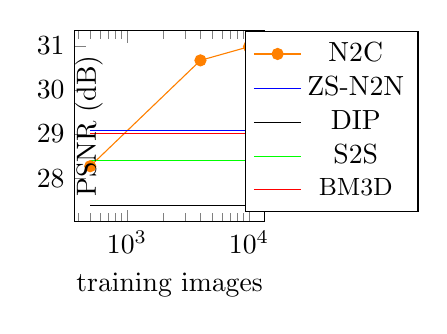
\begin{tikzpicture}
\begin{groupplot}[
xmode=log,
legend style={at={(1.35,1)},anchor=north}, 
legend style={cells={align=center}},
y label style={at={(axis description cs:0.20,0.5)},anchor=south},
group style={group size=1 by 1, horizontal sep=0.3cm, 
yticklabels at=edge left,
xticklabels at=edge bottom,
},
width=0.33\textwidth,height=0.33\textwidth, 
scaled x ticks=true,
every x tick label/.append style={alias=XTick,inner xsep=0pt},
every x tick scale label/.style={at=(XTick.base east),anchor=base west},
]
\nextgroupplot[xlabel = {training images},ylabel={PSNR (dB)}]
\addplot[mark=*,color=orange] coordinates { (500,28.27) (4000,30.67) (10000,30.98)};
\addlegendentry{{N2C}}
\addplot[mark=none,color=blue] coordinates {(500,29.07)  (10000,29.07) };
\addlegendentry{{ZS-N2N}}
\addplot[mark=none,color=black] coordinates {(500,27.38)  (10000,27.38) };
\addlegendentry{{DIP}}
\addplot[mark=none,color=green] coordinates {(500,28.39) (10000,28.39) };
\addlegendentry{{ S2S}}
\addplot[mark=none, color=red] coordinates {(500,29.02) (10000,29.02)};
\addlegendentry{{\small BM3D}}
\end{groupplot}
\end{tikzpicture}

\end{document}